% Options for packages loaded elsewhere
\PassOptionsToPackage{unicode}{hyperref}
\PassOptionsToPackage{hyphens}{url}
%
\documentclass[
  12pt,
]{article}
\author{}
\date{\vspace{-2.5em}}

\usepackage{amsmath,amssymb}
\usepackage{lmodern}
\usepackage{iftex}
\ifPDFTeX
  \usepackage[T1]{fontenc}
  \usepackage[utf8]{inputenc}
  \usepackage{textcomp} % provide euro and other symbols
\else % if luatex or xetex
  \usepackage{unicode-math}
  \defaultfontfeatures{Scale=MatchLowercase}
  \defaultfontfeatures[\rmfamily]{Ligatures=TeX,Scale=1}
\fi
% Use upquote if available, for straight quotes in verbatim environments
\IfFileExists{upquote.sty}{\usepackage{upquote}}{}
\IfFileExists{microtype.sty}{% use microtype if available
  \usepackage[]{microtype}
  \UseMicrotypeSet[protrusion]{basicmath} % disable protrusion for tt fonts
}{}
\makeatletter
\@ifundefined{KOMAClassName}{% if non-KOMA class
  \IfFileExists{parskip.sty}{%
    \usepackage{parskip}
  }{% else
    \setlength{\parindent}{0pt}
    \setlength{\parskip}{6pt plus 2pt minus 1pt}}
}{% if KOMA class
  \KOMAoptions{parskip=half}}
\makeatother
\usepackage{xcolor}
\IfFileExists{xurl.sty}{\usepackage{xurl}}{} % add URL line breaks if available
\IfFileExists{bookmark.sty}{\usepackage{bookmark}}{\usepackage{hyperref}}
\hypersetup{
  hidelinks,
  pdfcreator={LaTeX via pandoc}}
\urlstyle{same} % disable monospaced font for URLs
\usepackage[margin=1in]{geometry}
\usepackage{longtable,booktabs,array}
\usepackage{calc} % for calculating minipage widths
% Correct order of tables after \paragraph or \subparagraph
\usepackage{etoolbox}
\makeatletter
\patchcmd\longtable{\par}{\if@noskipsec\mbox{}\fi\par}{}{}
\makeatother
% Allow footnotes in longtable head/foot
\IfFileExists{footnotehyper.sty}{\usepackage{footnotehyper}}{\usepackage{footnote}}
\makesavenoteenv{longtable}
\usepackage{graphicx}
\makeatletter
\def\maxwidth{\ifdim\Gin@nat@width>\linewidth\linewidth\else\Gin@nat@width\fi}
\def\maxheight{\ifdim\Gin@nat@height>\textheight\textheight\else\Gin@nat@height\fi}
\makeatother
% Scale images if necessary, so that they will not overflow the page
% margins by default, and it is still possible to overwrite the defaults
% using explicit options in \includegraphics[width, height, ...]{}
\setkeys{Gin}{width=\maxwidth,height=\maxheight,keepaspectratio}
% Set default figure placement to htbp
\makeatletter
\def\fps@figure{htbp}
\makeatother
\setlength{\emergencystretch}{3em} % prevent overfull lines
\providecommand{\tightlist}{%
  \setlength{\itemsep}{0pt}\setlength{\parskip}{0pt}}
\setcounter{secnumdepth}{-\maxdimen} % remove section numbering
\newlength{\cslhangindent}
\setlength{\cslhangindent}{1.5em}
\newlength{\csllabelwidth}
\setlength{\csllabelwidth}{3em}
\newlength{\cslentryspacingunit} % times entry-spacing
\setlength{\cslentryspacingunit}{\parskip}
\newenvironment{CSLReferences}[2] % #1 hanging-ident, #2 entry spacing
 {% don't indent paragraphs
  \setlength{\parindent}{0pt}
  % turn on hanging indent if param 1 is 1
  \ifodd #1
  \let\oldpar\par
  \def\par{\hangindent=\cslhangindent\oldpar}
  \fi
  % set entry spacing
  \setlength{\parskip}{#2\cslentryspacingunit}
 }%
 {}
\usepackage{calc}
\newcommand{\CSLBlock}[1]{#1\hfill\break}
\newcommand{\CSLLeftMargin}[1]{\parbox[t]{\csllabelwidth}{#1}}
\newcommand{\CSLRightInline}[1]{\parbox[t]{\linewidth - \csllabelwidth}{#1}\break}
\newcommand{\CSLIndent}[1]{\hspace{\cslhangindent}#1}
\usepackage{setspace}
\doublespacing
\usepackage{lineno}
\linenumbers
\usepackage[belowskip=0pt,aboveskip=0pt]{caption} \usepackage{array} \usepackage{caption} \usepackage{graphicx} \usepackage{siunitx} \usepackage{colortbl} \usepackage{multirow} \usepackage{hhline} \usepackage{calc} \usepackage{tabularx} \usepackage{tabulary} \usepackage{threeparttable} \usepackage{wrapfig}
\usepackage{booktabs}
\usepackage{longtable}
\usepackage{array}
\usepackage{multirow}
\usepackage{wrapfig}
\usepackage{float}
\usepackage{colortbl}
\usepackage{pdflscape}
\usepackage{tabu}
\usepackage{threeparttable}
\usepackage{threeparttablex}
\usepackage[normalem]{ulem}
\usepackage{makecell}
\usepackage{xcolor}
\ifLuaTeX
  \usepackage{selnolig}  % disable illegal ligatures
\fi

\begin{document}

\newpage

\hypertarget{estimating-population-trends-with-stratified-random-sampling-under-the-pressures-of-climate-change}{%
\section{Estimating Population Trends with Stratified Random Sampling Under the Pressures of Climate Change}\label{estimating-population-trends-with-stratified-random-sampling-under-the-pressures-of-climate-change}}

Benjamin A. Levy\textsuperscript{1}, Christopher M. Legault\textsuperscript{2}, Timothy J. Miller\textsuperscript{2}, Elizabeth N. Brooks\textsuperscript{2}

\textsuperscript{1}Ben's Institution, USA\\
\textsuperscript{2}National Marine Fisheries Service, Northeast Fisheries Science Center, Woods Hole, MA, USA

Corresponding author: Ben Levy (\href{mailto:benjamin.levy@noaa.gov}{\nolinkurl{benjamin.levy@noaa.gov}})

Competing interests: The authors declare there are no competing interests.

{[}{[}Chris comments in double square brackets, search for them to see comments{]}{]}

\newpage

\hypertarget{abstract}{%
\subsection{Abstract}\label{abstract}}

An Abstract

\hypertarget{keywords}{%
\subsection{Keywords}\label{keywords}}

keyword 1, keyword 2

\newpage

\section{Introduction}

much of below is from \url{https://apps-nefsc.fisheries.noaa.gov/nefsc/ecosystem-ecology/}
or
\url{https://www.fisheries.noaa.gov/data-tools/fisheries-economics-united-states-data-and-visualizations}

\begin{itemize}
\tightlist
\item
  The eastern continental shelf is ecologically diverse and economically important
\end{itemize}

The Northeast United States continental shelf spans from the Outer Banks of North Carolina to the Gulf of Maine. The region covers over 250,000 km\(^2\) of ocean, extending over 200 km from shore in the largest areas in New England to just 30 km off shore in the southern regions. This ecologically diverse region contains approximately 18,000 vertebrate marine species. Commercial fisheries have been an important part of local economies for centuries. In 2019, New England fisheries produced \$22 billion in sales, which sustained over 200,000 jobs. Maintaining a healthy ecosystem is therefore vital to sustained ecological health and economic prosperity of the region. (NEFMC 2020)

\begin{itemize}
\tightlist
\item
  Bottom trawl survey is important for monitoring population trends
\end{itemize}

Fish stocks in this highly productive and economically important region are managed by the National Oceanic and Atmospheric Administration's (NOAA) Northeast Fisheries Science Center (NEFSC) in Woods Hole, Massachusetts. Federal scientists assess the health and abundance of each commercial fish stock using fishery-independent bottom trawl survey data that has been collected by NOAA throughout the region since 1963 (cite survey paper{[}{[}, some possible citations are \url{https://repository.library.noaa.gov/view/noaa/4825/noaa_4825_DS1.pdf} and T.S. Azarovitz 1981 A brief historical review of the Woods Hole Laboratory trawl survey time series. W.G. Doubleday, D. Rivard (Eds.), Bottom Trawl Surveys, Can. Spec. Pub. Fish. Aqua. Sci. No.~58 (1981), pp.~62-67{]}{]}). The survey uses a stratified random design where bottom trawl sampling takes place in predefined strata along the eastern continental shelf. The survey has created a rich time series data set with many uses including species-specific habitat identification, analysis of how environmental conditions influence species abundance, and estimating yearly species abundance trends to help inform stock assessments and ultimately quota limits \textbf{just listed a few uses of survey. change/add others?}.

The survey takes place twice each year- once in the spring and again in the fall. Since most spatial analyses and projections of future distributions typically assume a constant survey catchability and/or availability over time, NOAA's survey design includes sampling during approximately the same 2-3 week time period in each season.

\begin{itemize}
\tightlist
\item
  Climate change is happening
\end{itemize}

Due to a combination of climate change and shifts in circulation, the Northeast United States continental shelf has experienced rapid warming in recent decades, resulting in a shift in spatial distributions of many species. Since stock assessment models rely on accurate descriptions of population dynamics and contemporary patterns of spatial abundance, there is concern that rapid undocumented changes in spatial distributions of species will bias future stock assessments. The implication of this is that the bottom trawl survey is actually sampling the population during a different life cycle stage than was originally assumed {[}{[}I don't think the concern is about life cycle stage, but rather that the fish catchability or availability in the survey will change, thus changing the relationship between the index and the true population{]}{]}, which can lead to biased stock assessments. We are therefore interested in analyzing the impact of climate change on the accuracy of future stock assessment models as measured by NOAA's ongoing bottom-trawl survey along the East coast.

\begin{itemize}
\tightlist
\item
  say something about our study species? Past abundance history, biological characteristics, others? Maybe better suited in below section {[}{[}I think the specific species can wait for the methods section, just laying the groundwork here in the intro{]}{]}
\end{itemize}

\textbf{use more info from initial proposal}

\begin{itemize}
\item
  Fish are changing spatial distribution and have altered life stages (?) because of climate change {[}{[}see note above about catchability and availability{]}{]}
  NYE paper
\item
  Population indexing methods may be becoming biased as a result
\item
  Briefly describe our study to test this
\end{itemize}

To test the ability of the bottom trawl survey to track population trends under shifting environmental conditions, we construct spatial models for fish where movement depend on temperature preferences. We can then consider the impact of climate change by simulating scenarios with repeating temperature patterns and those where temperature increases on average over time. In both cases we analyze the ability of stratified random sampling to track population trends.

\section{Methods}

\begin{itemize}
\tightlist
\item
  Describe simulation study
\end{itemize}

We construct spatial models for Yellowtail Flounder, Atlantic Cod, and Haddock on {[}{[}Georges{]}{]} George's Bank, where movement of each species combine static species-specific habitat preferences with temperature preferences. Model dynamics are driven by a time series of temperature gradients that were estimated from data to create simulated data sets for each population where the true biomass is known. Using temperature gradients that repeat each year creates data sets with predictable, repeating spatial patterns, whereas using a temperature gradient that increases on average throughout the simulation leads to spatial distributions that shift over time {[}{[}and mimics the possible future in the region under climate change?{]}{]}. We conducting stratified random sampling on our simulation output to mimic the bottom trawl survey and compare the ability of contemporary indexing methods to track population trends.

\subsection{Population Model Formulation}

-- Used MixFishSim. Describe edits made to package

We use the R package \emph{MixFishSim} (MFS) to model our populations (Dolder et al. 2020). MFS is a discrete spatiotemporal simulation tool where users can model multiple species under varying environmental conditions. The package uses a delay-difference population model with discrete processes for growth, death, and recruitment of the population. We formulate the following inputs for the MFS package to address our research question. {[}{[}perhaps for discussion, but we should mention somewhere that MFS only tracks biomass not age structure, the latter is important for stock assessments but not considered in this paper{]}{]}

\emph{Study Area}

We obtained a shapefile for the 15 strata that comprise {[}{[}Georges Bank does not have an apostrophe, I made the same mistake when I started here{]}{]} George's Bank to use as our modeling environment. We discritized the region into a raster with 88 rows and 144 columns. Haddock inhabit all 15 strata in the domain, Cod inhabit 13 strata, and Yellowtail exist in 9 strata. Figure \ref{fig:strata-plot} shows the regions used in our models. {[}{[}can mention that the different strata are based on biological differences among the species, possibly add that there are multiple stocks for all three species and the delineations among the stocks differ by species{]}{]}

\begin{figure}

{\centering 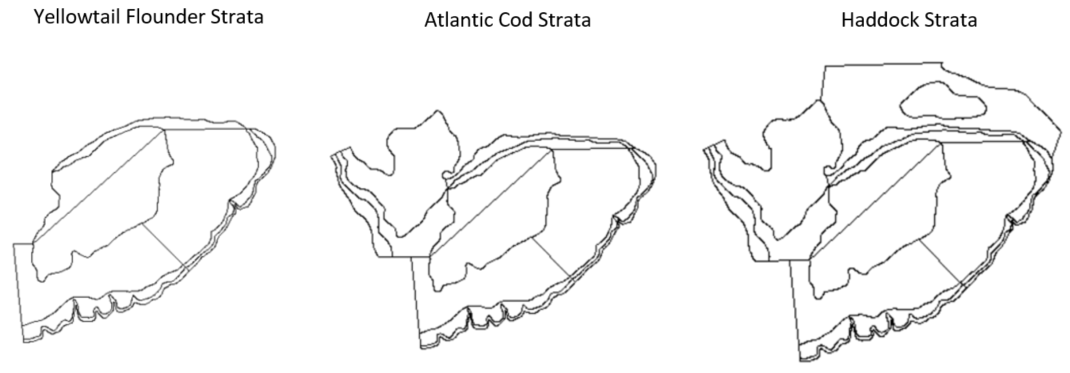
\includegraphics[width=0.95\linewidth]{Images/Strata} 

}

\caption{Strata inhabited by each species in our population models.}\label{fig:strata-plot}
\end{figure}

\emph{Population Dynamics and Recruitment}

The time step for our models is one week. MFS uses a modified two-stage Deriso-Schnute delay difference equation that models the biomass in each cell in our study area (Dolder et al. 2020). Individual terms in the formulation account for growth of mature adults, natural and fishing mortality, and the addition of new recruits. {[}{[}not sure we need to highlight the recruitment model, might be able to just use the table because Bev-Holt formulation is well known in fisheries{]}{]} We chose to represent recruitment in the model using a Beverton-Holt formulation \textbf{cite}. Recruitment is a function of the adult biomass that existed in the previous year and is added to the population incrementally throughout each species' predefined spawning period. Parameter inputs were either obtained from the literature or chosen to produce desired model dynamics. A full list of parameters used in our model can be seen below in Tables \ref{paramsALL} and \ref{tab:paramsSCENARIOS}.

\emph{Movement}

The package was designed to generate theoretical habitat preferences using Gaussian Random Fields that combine with hypothetical temperature gradients to drive the probability of movement from cell \(I\) to cell \(J\) using the formulation

\begin{align}
Pr(C_{wk+1}=J|C_{wk}=I) = \frac{e^{-\lambda \cdot d_{I,J}}\cdot(Hab^2_{J,s} \cdot Tol_{J,s,wk})}{\sum^C_{c=1}e^{-\lambda \cdot d} \cdot (Hab^2_{c,s} \cdot Tol_{c,s,wk})},
\label{moveP}
\end{align}

where

\(e^{-\lambda \cdot d_{I,J}}\) accounts for distance between cells \(I\) and \(J\),

\(Hab^2_{J,s}\) is the static habitat value for species \(s\) in cell \(J\), and

\(Tol_{c,s,wk}\) is the value from normally distributed temperature tolerance for species \(s\) in cell \(c\) in week \(wk\).

The following sections describe how we formulated the habitat and temperature components to model real species on the northeast continental shelf.

\emph{Habitat Input}

Species-specific habitat preferences were derived using the \emph{lrren} tool from the R package \emph{envi} (Buller 2022) to create a niche model for each species. The \emph{lrren} tool estimates an ecological niche using the relative risk function by relating presence/absence data to two covariate predictors. We used bottom trawl point data in from 2009-2021 as our presence/absence input by using a value of 0 for any tow that failed to catch the given species and weighting a successful catch by the biomass of the given tow {[}{[}I don't think we need to cite the trawl data because we said we were using trawl data above{]}{]} \textbf{cite trawl data?}. We combined data from both the fall and spring surveys to obscure the influence of temperature so that the niche model would instead infer habitat preferences. Depth and mean sediment size were used as our covariate predictors. Estimated depth for the region was obtained from FVCOM (Chen et al. 2006). The mean sediment size raster was interpolated in ArcMap using the natural neighbor interpolation method {[}{[}citing ArcMap should suffice{]}{]} \textbf{cite arcmap or more?} using point data collected by the United States Geologic Survey (USGS) (McMullen et al. n.d.). Since the values in \(Hab^2_{J,s}\) are required to be between 0 and 1, we transform the spatial estimates from \emph{lrren} to fall between these bounds. See Figure \ref{fig:hab-plot1} for a visual representation of this process being applied to Cod. Figure \ref{fig:hab-plot} depicts habitat preferences \(Hab^2_{J,s}\) for each species.

\begin{figure}

{\centering 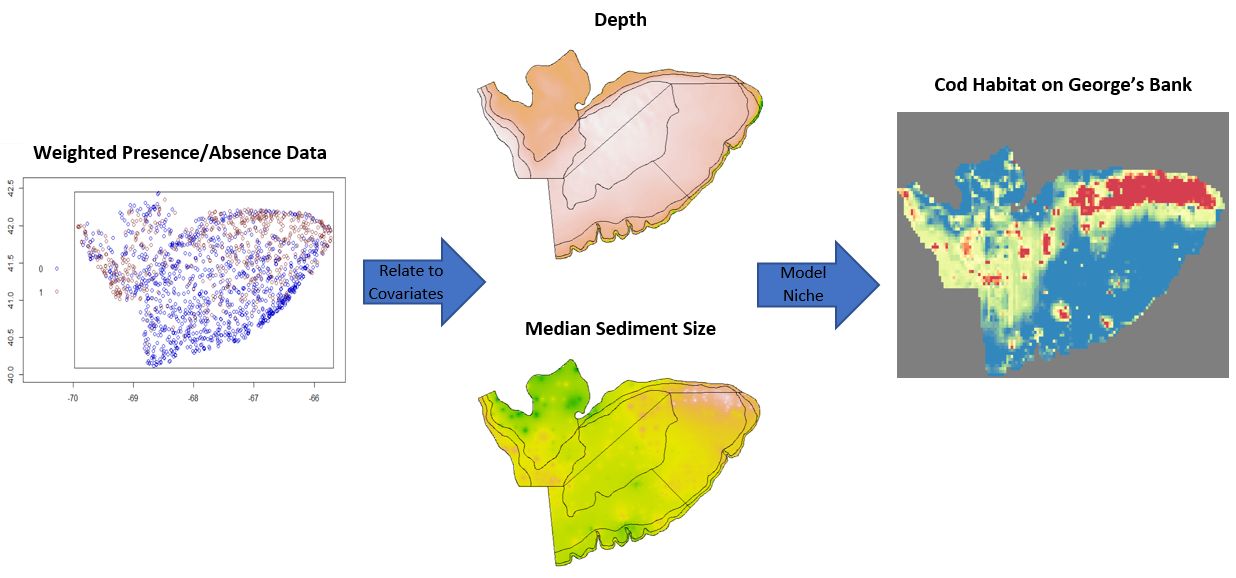
\includegraphics[width=0.95\linewidth]{Images/hab_snip3} 

}

\caption{Visual representation of niche model for Cod.}\label{fig:hab-plot1}
\end{figure}

\begin{figure}

{\centering 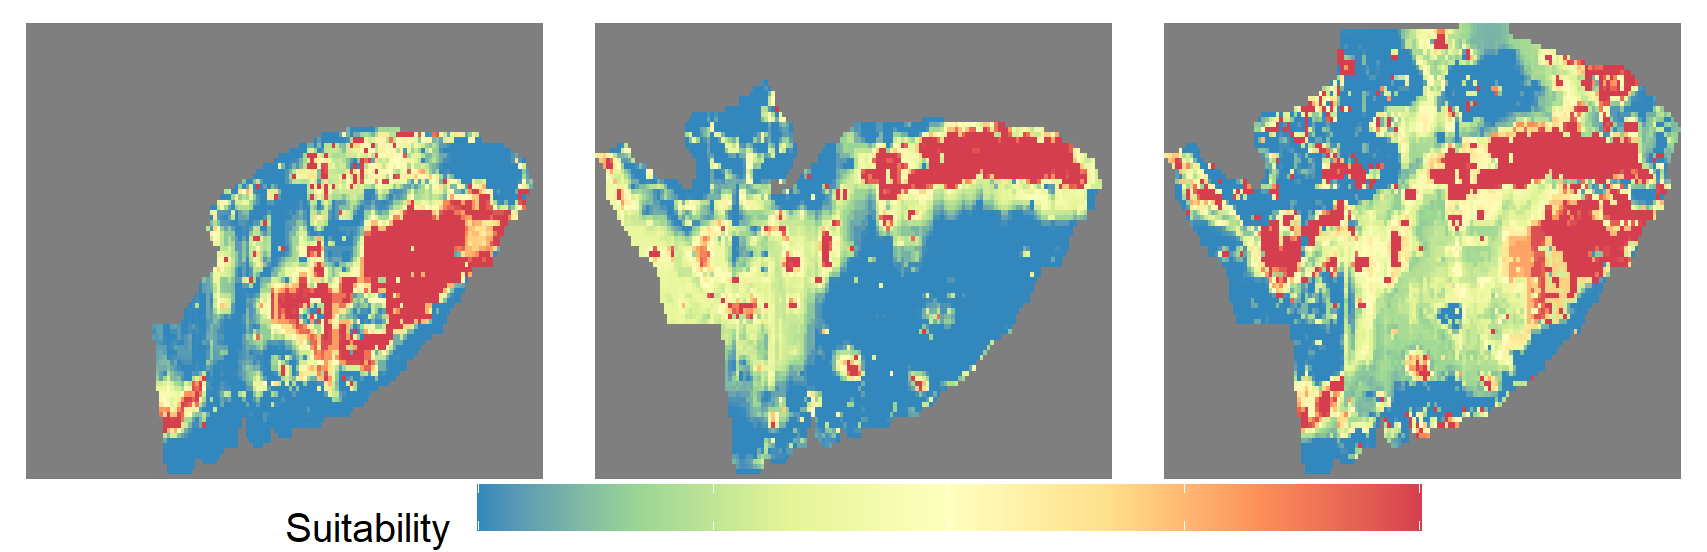
\includegraphics[width=0.95\linewidth]{Images/Habitat_3species} 

}

\caption{Static habitat preferences for each species in our population models (Yellotwtail, Cod, Haddock).}\label{fig:hab-plot}
\end{figure}

\emph{Temperature Input}

Each species is assumed to have normally distributed temperature preferences (\(N(\mu,\sigma)\)). We assume Yellowtail Flounder's preferences are \(N(8.75,4.25)\), while Haddock and Cod have preferences \(N(9,4)\). We chose these values by combining information in the literature with temperatures recorded in the bottom trawl survey. Weekly estimated temperature data for the region for 2012 was obtained from FVCOM (Chen et al. 2006). We chose 2012 because the data displayed an average temperature pattern that consistently oscillated between maximum and minimum temperature values. This data was also transform to create an oscillating pattern that increases 5 degrees Celsius on average over the duration of the simulation. \textbf{show images of temperature and/or and/or temp videos??? and/or average temperature oscillations?}{[}{[}as we discussed, one plot here comparing average temperatures for constant and increasing scenarios in the paper, one or more animations in supplemental materials{]}{]}

--Describe difference between increasing and constant temperature scenarios (images?)

In equation (1), \(Hab^2_{J,s}\) is constant for the duration of the simulation, while \(Tol_{c,s,wk}\) changes each week. Using a temperature gradient that repeats every 52 weeks produces the same spatial preferences in a given week each year, resulting in consistent spatial biomass patterns. Scenarios where the temperature increases over time creates spatial preferences that evolve as the water warms, producing spatial biomass patterns that shift in a given week over the duration of the simulation. Thus, stratified random samples in scenarios with a repeating temperature pattern will have constant survey catchability and availability over time, which may not be true for increasing temperature scenarios due to evolving spatial preferences. {[}{[}may want to mention here or in the discussion that we used repeating 2012 to simplify the simulations and reduce the number of factors explored that would have occurred with different annual cycles{]}{]}

-- Describe each scenario that is considered

We consider 20 year simulations under three population parameter scenarios for each of our three species- a scenario where parameters result in each population increasing over time, one where the populations are relatively constant over time, and a scenario where the parameter combination results in each population decreasing over time. Each of these three scenarios is paired with a temperature gradient that repeats as well as one that increasing roughly 5 degrees Celsius {[}{[}need some justification for this large change, wanted to be extreme because if the extreme doesn't make a difference, then more reasonable increases wouldn't make a difference{]}{]} over the duration of the 20 year simulation. We therefore simulate a total of 6 scenarios. \textbf{show line plot of population for each?}

\emph{Simulating Bottom Trawl Survey and Population Indexing}

-Describe post hoc sampling process and how data is used

After each simulation is complete, we mimic the bottom trawl survey by conducting stratified random sampling in each inhabited strata twice each year. We sample in the same weeks that the Spring and Fall surveys take place and the number of the samples taken in each strata reflect true values. {[}{[}need to make sure that we don't lose sight of random samlping with the following sentences{]}{]} Most strata contain enough cells to sample a unique location in each survey over the duration of the simulation. For smaller strata we must repeat some sample locations. We then use the biomass collected from our samples in contemporary population indexing methods to estimate population trends. Knowing the true population values in our simulations allows us to compare the error calculated from each estimation method.{[}{[}should we mention here or later that we did both with and without measurement error analyses?{]}{]}

--Stratified mean vs VAST with and without covariates

{[}{[}could use an intro sentence here to distinguish design-based (stratified mean) and model-based (VAST) estimators{]}{]} We compare the yearly estimated of abundance obtained from the stratified mean to estimates obtained from the Vector-Autoregressive Spatio-temporal (VAST) model. The stratified mean is a typical survey-based approach that scales individual samples to the strata-level by considering the area of each strata, before scaling to the region-level based on the relative size of each strata. VAST is a spatio-temporal statistical framework that models both abundance (biomass) and probability of occurrence (presence/absence). If desired, VAST also allows users to include covariate data to better inform the model. Covariates can be static (eg. habitat preferences) or dynamics (eg. temperature). The stratified mean calculations are straightforward and quick, while VAST models require numerous user inputs and take on the order of hours to complete.{[}{[}may want to highlight the potential of VAST with covariates to address the climate change issue here as the reason we are doing these simulations{]}{]}

We follow the advice given in (Thorson 2019) to build VAST models to estimate biomass on {[}{[}Georges{]}{]} George's Bank using stratified mean samples from our model output. In addition to exploring different link functions and assumed distributions, our VAST model-building process included testing the impact of including spatial and/or spatio-temporal variation in our models, considering varying number of knots in our mesh, and testing different forms of temporal correlation. We also carried out the same process both including covariates in our model as well as running models without covariate information. We considered covariates in the form of dynamic temperature values and/or static habitat values from our population model. When using covariates we ultimately decided to provide the most information to the model by including both covariates for both linear predictors. Since we know the true population values in our models we calculate the absolute error of each VAST estimate to compare between potential settings. Through this process, and in consultation with the VAST package creator, we determined setting that allowed VAST models to converge for all of our scenarios while also providing the lowest absolute error values. Settings for our VAST models can be seen in Table ???.

Our goal is to determine indexing approaches and settings that are robust to future environmental conditions and resulting spatial biomass patterns. An underlying assumption in all indexing methods that individual random samples combine to accurately represent true abundance by a) sampling all strata in which the population exists and b) low enough noise level in the samples to allow for a discernible pattern. This assumption can be questioned given enough noise in the sampling process \textbf{cite?} and/or shifting spatial preferences driven by climate change causing a population to move into a previously uninhabited strata. To simulate the impact of noise, indexing estimates after adding noise to our samples versus those using the true sampling values. To evaluate the effect of populations moving into new habitat, we compare indexing estimates using samples from all strata versus those that only include a subset of the full spatial domain for each species. {[}{[}may need to spell the aspect of reduced spatial domain a bit more because it might be confusing to readers who are expected us to just add areas around the current ones instead of reducing the strata{]}{]}

When combining population trends for each species, differing temperature scenarios, altering seasons, and sampling possibilities (noise, strata, covariates) there are a large number of scenario combinations to consider. The columns in Table COMBOS show the choices that define each scenario.

Table COMBOS Each index estimate chooses one condition from each of the following columns. There are \(3*3*2*2*2*2*2=288\) VAST model combinations and \(3*3*2*2*2=144\) stratified mean estimates.

\begin{longtable}[]{@{}
  >{\raggedright\arraybackslash}p{(\columnwidth - 12\tabcolsep) * \real{0.14}}
  >{\raggedright\arraybackslash}p{(\columnwidth - 12\tabcolsep) * \real{0.14}}
  >{\raggedright\arraybackslash}p{(\columnwidth - 12\tabcolsep) * \real{0.14}}
  >{\raggedright\arraybackslash}p{(\columnwidth - 12\tabcolsep) * \real{0.14}}
  >{\raggedright\arraybackslash}p{(\columnwidth - 12\tabcolsep) * \real{0.14}}
  >{\raggedright\arraybackslash}p{(\columnwidth - 12\tabcolsep) * \real{0.18}}
  >{\raggedright\arraybackslash}p{(\columnwidth - 12\tabcolsep) * \real{0.14}}@{}}
\toprule
\begin{minipage}[b]{\linewidth}\raggedright
Species
\end{minipage} & \begin{minipage}[b]{\linewidth}\raggedright
Population Trend
\end{minipage} & \begin{minipage}[b]{\linewidth}\raggedright
Temperature Scenario
\end{minipage} & \begin{minipage}[b]{\linewidth}\raggedright
Strata Included
\end{minipage} & \begin{minipage}[b]{\linewidth}\raggedright
Noise in Data
\end{minipage} & \begin{minipage}[b]{\linewidth}\raggedright
Covariates (VAST only)
\end{minipage} & \begin{minipage}[b]{\linewidth}\raggedright
Season
\end{minipage} \\
\midrule
\endhead
Yellowtail & Increasing & Repeating & All strata & No Noise & No Covariates & Spring \\
Cod & Constant & Increasing 5\(^{\circ}\) & Subset & Yes Noise & Temp + Habitat & Fall \\
Haddock & Decreasing & & & & & \\
\bottomrule
\end{longtable}

\section{Results}

The goal of our project was to analyze how well contemporary population indexing methods can track population trends under a host of conditions, as depicted in Table COMBOS. Historically, Atlantic Cod has seen significant decline over the last XXX years while Haddock has increased in abundance in recent year {[}{[}can cite the 2022 management track assessments, see \url{https://apps-nefsc.fisheries.noaa.gov/saw/sari.php} for when the document becomes available{]}{]} \textbf{cite}. For this reason we compare indexing estimates using stratified random samples from decreasing population scenarios for Cod (see Table ???) and increasing population scenarios for Haddock (see Table ???). To provide a comprehensive analysis of population indexing methods we consider all possible scenario combinations for Yellowtail Flounder (see Table ???).

General themes that exist in Tables X, Y and Z are that VAST estimates provide lower errors relative to those derived from the stratified mean, with VAST models that include covariate information providing the lowest overall errors. We also see individual cases where the stratified mean produced the lowest absolut error and instances where including covarites in VAST models actually increase the absolute error. When we reduce the number of strata that are included in indexing calculations to simulation species shifting into new territory, we typically see an increase in absolute error {[}{[}as expected{]}{]}, though there are some scenarios where the impact is minimal.

In the Cod results, when using reduced strata adding covariates produces worst VAST results (though still better than stratified mean). VAST without covariates much worse than stratified mean in fall with increasing temperature and all strata, but adding covariates corrects this.

For Haddock, VAST has a particularly hard time in spring regularly producing larger errors than the stratified mean with added covariates only improving to the level of the stratified mean. VAST shows improved results in fall relative to the stratified mean with added covaraites producing extremely low errors in some cases.

In considering the Yellowtail Flounder results in Table XXX, we can see VAST estimates generally provide lower errors relative to those derived from the stratified mean, with models that include covariate information typically providing the lowest errors. However, there are several instances in which VAST failed to provide improved abundance estimates during the fall season without covariate information, producing the largest errors seen in the Table. These errors are corrected by including covariate information allowing for an improved VAST estimate that are significantly lower than their stratified mean counterparts.

{[}{[}We'll want to expand the results section to focus on the impact of each factor one at at time within each species. This will be a bit dull, but it is important to walk through the results in words to ensure that readers get the message. They can of course examine the tables in detail and draw their own conclusions, but we should put our interpretation down on paper.{]}{]}

\begin{table}

\caption{\label{tab:unnamed-chunk-1}Yellowtail error results}
\centering
\begin{tabular}[t]{l|l|l|l|l|l|l|l|l|l|l}
\hline
X & X.1 & X.2 & X.3 & X.4 & Constant.Population & X.5 & Increasing.Population & X.6 & Decreasing.Population & X.7\\
\hline
Temp & Covariate & Strata & Noise & season & Stratified Mean & VAST Estimate & Stratified Mean & VAST Estimate & Stratified Mean & VAST Estimate\\
\hline
const & no cov & all & no & spring & 0.21 & 0.11 & 0.16 & 0.13 & 0.23 & 0.08\\
\hline
const & no cov & all & yes & spring & 0.25 & 0.16 & 0.22 & 0.21 & 0.27 & 0.11\\
\hline
const & w/ cov & all & no & spring & 0.21 & 0.07 & 0.16 & 0.06 & 0.23 & 0.06\\
\hline
const & w/ cov & all & yes & spring & 0.25 & 0.08 & 0.22 & 0.07 & 0.27 & 0.07\\
\hline
const & no cov & all & no & fall & 0.32 & 0.68 & 0.34 & 0.36 & 0.41 & 0.81\\
\hline
const & no cov & all & yes & fall & 0.31 & 0.77 & 0.46 & 0.44 & 0.44 & 1.09\\
\hline
const & w/ cov & all & no & fall & 0.32 & 0.08 & 0.34 & 0.08 & 0.41 & 0.08\\
\hline
const & w/ cov & all & yes & fall & 0.31 & 0.11 & 0.46 & 0.17 & 0.44 & 0.18\\
\hline
const & no cov & reduced & no & spring & 0.27 & 0.19 & 0.2 & 0.15 & 0.25 & 0.19\\
\hline
const & no cov & reduced & yes & spring & 0.26 & 0.15 & 0.22 & 0.11 & 0.3 & 0.16\\
\hline
const & w/ cov & reduced & no & spring & 0.27 & 0.19 & 0.2 & 0.17 & 0.25 & 0.19\\
\hline
const & w/ cov & reduced & yes & spring & 0.26 & 0.14 & 0.22 & 0.13 & 0.3 & 0.16\\
\hline
const & no cov & reduced & no & fall & 0.47 & 0.25 & 0.41 & 0.11 & 0.55 & 0.24\\
\hline
const & no cov & reduced & yes & fall & 0.49 & 0.36 & 0.46 & 0.21 & 0.53 & 0.36\\
\hline
const & w/ cov & reduced & no & fall & 0.47 & 0.19 & 0.41 & 0.22 & 0.55 & 0.23\\
\hline
const & w/ cov & reduced & yes & fall & 0.49 & 0.17 & 0.46 & 0.19 & 0.53 & 0.24\\
\hline
increasing & no cov & all & no & spring & 0.28 & 0.11 & 0.32 & 0.13 & 0.22 & 0.15\\
\hline
increasing & no cov & all & yes & spring & 0.28 & 0.15 & 0.34 & 0.16 & 0.26 & 0.17\\
\hline
increasing & w/ cov & all & no & spring & 0.28 & 0.06 & 0.32 & 0.07 & 0.22 & 0.07\\
\hline
increasing & w/ cov & all & yes & spring & 0.28 & 0.12 & 0.34 & 0.1 & 0.26 & 0.1\\
\hline
increasing & no cov & all & no & fall & 0.51 & 1.26 & 0.3 & 0.66 & 0.28 & 1.06\\
\hline
increasing & no cov & all & yes & fall & 0.5 & 1.38 & 0.39 & 0.71 & 0.25 & 1.1\\
\hline
increasing & w/ cov & all & no & fall & 0.51 & 0.23 & 0.3 & 0.21 & 0.28 & 0.15\\
\hline
increasing & w/ cov & all & yes & fall & 0.5 & 0.28 & 0.3 & 0.37 & 0.25 & 0.2\\
\hline
increasing & no cov & reduced & no & spring & 0.31 & 0.17 & 0.4 & 0.33 & 0.32 & 0.14\\
\hline
increasing & no cov & reduced & yes & spring & 0.29 & 0.19 & 0.41 & 0.26 & 0.29 & 0.15\\
\hline
increasing & w/ cov & reduced & no & spring & 0.31 & 0.17 & 0.4 & 0.3 & 0.32 & 0.22\\
\hline
increasing & w/ cov & reduced & yes & spring & 0.29 & 0.15 & 0.41 & 0.25 & 0.29 & 0.21\\
\hline
increasing & no cov & reduced & no & fall & 0.64 & 0.75 & 0.7 & 0.49 & 0.54 & 0.6\\
\hline
increasing & no cov & reduced & yes & fall & 0.66 & 0.89 & 0.69 & 0.48 & 0.53 & 0.62\\
\hline
increasing & w/ cov & reduced & no & fall & 0.64 & 0.2 & 0.7 & 0.53 & 0.54 & 0.31\\
\hline
increasing & w/ cov & reduced & yes & fall & 0.66 & 0.13 & 0.69 & 0.5 & 0.53 & 0.32\\
\hline
\end{tabular}
\end{table}

\begin{table}

\caption{\label{tab:unnamed-chunk-1}Cod error results}
\centering
\begin{tabular}[t]{l|l|l|l|r|r|r}
\hline
Temp & Strata & Noise & season & VAST.No.Cov & VAST.w..Cov & Stratified.Mean\\
\hline
constant & all & no & spring & 0.11 & 0.12 & 0.36\\
\hline
constant & all & yes & spring & 0.12 & 0.15 & 0.35\\
\hline
constant & all & no & fall & 0.19 & 0.05 & 0.49\\
\hline
constant & all & yes & fall & 0.30 & 0.23 & 0.41\\
\hline
constant & reduced & no & spring & 0.17 & 0.24 & 0.41\\
\hline
constant & reduced & yes & spring & 0.20 & 0.23 & 0.46\\
\hline
constant & reduced & no & fall & 0.21 & 0.33 & 0.60\\
\hline
constant & reduced & yes & fall & 0.18 & 0.31 & 0.58\\
\hline
increasing & all & no & spring & 0.12 & 0.15 & 0.25\\
\hline
increasing & all & yes & spring & 0.19 & 0.19 & 0.27\\
\hline
increasing & all & no & fall & 0.76 & 0.13 & 0.45\\
\hline
increasing & all & yes & fall & 0.89 & 0.33 & 0.44\\
\hline
increasing & reduced & no & spring & 0.14 & 0.22 & 0.32\\
\hline
increasing & reduced & yes & spring & 0.15 & 0.21 & 0.29\\
\hline
increasing & reduced & no & fall & 0.60 & 0.31 & 0.54\\
\hline
increasing & reduced & yes & fall & 0.62 & 0.32 & 0.53\\
\hline
\end{tabular}
\end{table}

\begin{table}

\caption{\label{tab:unnamed-chunk-1}Haddock error results}
\centering
\begin{tabular}[t]{l|l|l|l|r|r|r|l|l}
\hline
Temp & Strata & Noise & season & VAST.No.Cov & VAST.w..Cov & Stratified.Mean & X & X.1\\
\hline
const & all & no & spring & 0.49 & 0.18 & 0.18 & NA & \\
\hline
const & all & yes & spring & 0.73 & 0.43 & 0.21 & NA & Haddock\\
\hline
const & all & no & fall & 0.28 & 0.05 & 0.26 & NA & Increasing Population\\
\hline
const & all & yes & fall & 0.41 & 0.06 & 0.27 & NA & \\
\hline
const & reduced & no & spring & 0.34 & 0.35 & 0.45 & NA & \\
\hline
const & reduced & yes & spring & 0.30 & 0.33 & 0.46 & NA & \\
\hline
const & reduced & no & fall & 0.36 & 0.48 & 0.54 & NA & \\
\hline
const & reduced & yes & fall & 0.33 & 0.46 & 0.52 & NA & \\
\hline
increasing & all & no & spring & 0.25 & 0.05 & 0.26 & NA & \\
\hline
increasing & all & yes & spring & 0.30 & 0.06 & 0.31 & NA & \\
\hline
increasing & all & no & fall & 0.89 & 0.23 & 0.40 & NA & \\
\hline
increasing & all & yes & fall & 1.04 & 0.35 & 0.42 & NA & \\
\hline
increasing & reduced & no & spring & 0.32 & 0.40 & 0.44 & NA & \\
\hline
increasing & reduced & yes & spring & 0.38 & 0.37 & 0.37 & NA & \\
\hline
increasing & reduced & no & fall & 0.44 & 0.64 & 0.72 & NA & \\
\hline
increasing & reduced & yes & fall & 0.42 & 0.62 & 0.70 & NA & \\
\hline
\end{tabular}
\end{table}

\section{Discussion}

{[}{[} some things that I think we'll need to address, in addition to those mentioned above are (in no particular order):
number of simulations done for each scenario - time required to do them and analyses
pros and cons of using VAST with covariates in a changing environment
implications for current practice of using stratified mean (not horrible, but might be able to do better with model-based using covariates if enviro changing, note we don't want to say stratified mean should not be used because that will draw a lot of tomato throwing)
future work - some of the ideas we've discussed already could be mentioned
limitations to our study{]}{]}

\section{Acknowledgements}

{[}{[}we should thank Jim (obviously), but also those who helped you with the habitat data and others? also should note that funding provided by Climate-Groundfish source (I'll dig up the official name of the funding source){]}{]}

\hypertarget{data-and-code-availability}{%
\subsection{Data and Code Availability}\label{data-and-code-availability}}

All data and code used in this work are available at \url{https://github.com/cmlegault/IBMWG}. {[}{[}need to update this{]}{]}

\hypertarget{references}{%
\subsection{References}\label{references}}

\hypertarget{refs}{}
\begin{CSLReferences}{1}{0}
\leavevmode\vadjust pre{\hypertarget{ref-envi}{}}%
Buller, I.D. 2022. Envi: Environmental interpolation using spatial kernel density estimation. The Comprehensive R Archive Network. doi:\href{https://doi.org/10.5281/zenodo.5347826}{10.5281/zenodo.5347826}.

\leavevmode\vadjust pre{\hypertarget{ref-chen2006unstructured}{}}%
Chen, C., Beardsley, R.C., Cowles, G., Qi, J., Lai, Z., Gao, G., and others. 2006. An unstructured grid, finite-volume coastal ocean model: FVCOM user manual. SMAST/UMASSD: 6--8.

\leavevmode\vadjust pre{\hypertarget{ref-dolder2020highly}{}}%
Dolder, P.J., Minto, C., Guarini, J.-M., and Poos, J.J. 2020. Highly resolved spatiotemporal simulations for exploring mixed fishery dynamics. Ecological Modelling \textbf{424}: 109000. Elsevier.

\leavevmode\vadjust pre{\hypertarget{ref-mcmullen2005usgs}{}}%
McMullen, K., Paskevich, V., and Poppe, L. (n.d.). USGS east-coast sediment analysis: Procedures, database, and GIS data. US Geological Survey Open-File Report \textbf{2005}: 1001.

\leavevmode\vadjust pre{\hypertarget{ref-nefmc20}{}}%
NEFMC. 2020. {Northeast skate complex fishery management plan. Amendment 5 discussion document}. {Available online at https://www.nefmc.org/library/amendment-5-3}.

\leavevmode\vadjust pre{\hypertarget{ref-thorson2019guidance}{}}%
Thorson, J.T. 2019. Guidance for decisions using the vector autoregressive spatio-temporal (VAST) package in stock, ecosystem, habitat and climate assessments. Fisheries Research \textbf{210}: 143--161. Elsevier.

\end{CSLReferences}

\pagebreak

\hypertarget{tables}{%
\subsection{Tables}\label{tables}}

\pagebreak

Table 1. Parameters used in all population models.

\begin{longtable}[]{@{}lllllll@{}}
\toprule
Parameter & Description & Unit & Yellowtail & Cod & Haddock & Source \\
\midrule
\endhead
\(\rho\) & Ford's growth coefficient & wk\(^{-1}\) & 4.48 & 4.43 & 4.49 & \\
\(M\) & Natural Mortality & wk\(^{-1}\) & 0.2064 & 0.2728 & 0.3340 & \\
\(W_R\) & Weight of fully recruited fish & kg & 0.39 & 2.95 & 1.12 & \\
\(W_{R-1}\) & Weight of pre-recruit fish & kg & 0.13 & 0.39 & 0.19 & \\
\(\sigma^2\) & Variance in recruited fish & kg\(^2\) & 0.55 & 0.55 & 0.55 & \\
\(\lambda\) & Decay rate for movement & - & 0.7 & 0.7 & 0.7 & \\
\(Spwn_s\) & Spawning weeks for species \(s\) & wk & 9-12 & 8-13 & 11-14 & \\
\(Rec_s\) & Recruitment weeks for species \(s\) & wk & 9-12 & 8-13 & 11-14 & \\
\bottomrule
\end{longtable}

\begin{table}
 
 \caption{\label{tab:paramsALL2}Parameters used in all population models.}
 \centering
 \fontsize{10}{12}\selectfont
 \begin{tabular}[t]{lllllll}
 \toprule
 Parameter & Description & Unit & Yellowtail & Cod & Haddock & Source\\
 \midrule
 <U+03C1> & Ford's growth coefficient & 1/wk & 4.48 & 4.43 & 4.49 & NA\\
 M & Natural mortality & 1/wk & 0.2064 & 0.2728 & 0.334 & NA\\
 W1 & Weight of fully recruited fish & kg & 0.39 & 2.95 & 1.12 & NA\\
 W2 & Weight of pre-recruit fish & kg & 0.13 & 0.39 & 0.19 & NA\\
 sigma & Variance in recruited fish & kg*kg & 0.55 & 0.55 & 0.55 & NA\\
 \addlinespace
 lambda & Decay rate for movement & - & 0.7 & 0.7 & 0.7 & NA\\
 spwn & Spawning weeks for species s & wks & 9-12 & 8-13 & 11-14 & NA\\
 rec & Recruitment weeks for species s & wks & 9-12 & 8-13 & 11-14 & NA\\
 \bottomrule
 \end{tabular}
 \end{table}

\begin{table}

\caption{\label{tab:paramsSCENARIOS}Parameters used in population models for each scenario.}
\centering
\fontsize{10}{12}\selectfont
\begin{tabular}[t]{llllll}
\toprule
Parameter & Description & Unit & Yellowtail & Cod & Haddock\\
\midrule
\addlinespace[0.3em]
\multicolumn{1}{l}{\textbf{Constant Population}}\\
\hspace{1em}M+F & Adjusted Mortality (Natural + Fishing) & 1/wk & 0.764 & 0.83 & 0.309\\
\hspace{1em}P0 & Initial Biomass & kg & 3190 & 21500 & \vphantom{1} 180000\\
\hspace{1em}a & Max recruitment rate & kg & 30400 & 27900 & 73600\\
\hspace{1em}ß & Recruitment half saturation value & kg & 4300 & 10500 & 40500\\
\addlinespace[0.3em]
\multicolumn{1}{l}{\textbf{Decreasing Population}}\\
\hspace{1em}M+F & Adjusted Mortality (Natural + Fishing) & 1/wk & 0.764 & 0.623 & 0.334\\
\hspace{1em}P0 & Initial Biomass & kg & 50000 & 21500 & 180000\\
\hspace{1em}a & Max recruitment rate & kg & 1.07e+12 & 3.89e+08 & 4.97e+08\\
\hspace{1em}ß & Recruitment half saturation value & kg & 2.3e+12 & 9.8e+08 & 2.08e+09\\
\addlinespace[0.3em]
\multicolumn{1}{l}{\textbf{Increasing Population}}\\
\hspace{1em}M+F & Adjusted Mortality (Natural + Fishing) & 1/wk & 0.564 & 0.372 & 0.134\\
\hspace{1em}P0 & Initial Biomass & kg & 3190 & 21500 & 180000\\
\hspace{1em}a & Max recruitment rate & kg & 40000 & 45000 & 1e+05\\
\hspace{1em}ß & Recruitment half saturation value & kg & 43000 & 62800 & 405000\\
\bottomrule
\end{tabular}
\end{table}

Table XX. Parameters used in all VAST models.

\begin{longtable}[]{@{}
  >{\raggedright\arraybackslash}p{(\columnwidth - 4\tabcolsep) * \real{0.13}}
  >{\raggedright\arraybackslash}p{(\columnwidth - 4\tabcolsep) * \real{0.53}}
  >{\raggedright\arraybackslash}p{(\columnwidth - 4\tabcolsep) * \real{0.33}}@{}}
\toprule
\begin{minipage}[b]{\linewidth}\raggedright
Parameter
\end{minipage} & \begin{minipage}[b]{\linewidth}\raggedright
Description
\end{minipage} & \begin{minipage}[b]{\linewidth}\raggedright
Input/Value
\end{minipage} \\
\midrule
\endhead
\emph{ObsModel} & Link function and assumed distribution & c(10,2) \\
FieldCOnfig & Specified spatial and/or spatio-temporal variation in predictors & c(Omega1=0, Epsilon1=0, Omega2=1, Epsilon2=1) \\
RhoConfig & Specifying whether intercepts or spatio-temporal variation is structured among time intervals & c(Beta1=3, Beta2=3, Epsilon1=0, Epsilon2=4) \\
X1\_formula & Right-sided formula affecting the 1st linear predictor & X1\_formula = \textasciitilde{} poly(Temp, degree=2 ) \\
X2\_formula & Right-sided formula affecting the 2nd linear predictor & X2\_formula = \textasciitilde{} poly(Temp, degree=2 ) + poly(Habitat, degree=2 ) \\
\bottomrule
\end{longtable}

\begin{table}
\centering\begingroup\fontsize{10}{12}\selectfont

\begin{tabular}{l|l|l|l|l|l|r|r}
\hline
Temp & Covariate & Strata & Noise & Season & Scenario & Stratified Mean & VAST Estimate\\
\hline
\multicolumn{1}{l}{\textbf{all}}\\
\hline
\multicolumn{1}{l}{\textbf{Constant Population}}\\
\hline
\hspace{1em}\hspace{1em}constant & no cov & all & no & spring & Constant Population & 0.21 & 0.11\\
\hline
\hspace{1em}\hspace{1em}constant & no cov & all & yes & spring & Constant Population & 0.25 & 0.16\\
\hline
\hspace{1em}\hspace{1em}constant & w/ cov & all & no & spring & Constant Population & 0.21 & 0.07\\
\hline
\hspace{1em}\hspace{1em}constant & w/ cov & all & yes & spring & Constant Population & 0.25 & 0.08\\
\hline
\hspace{1em}\hspace{1em}constant & no cov & all & no & fall & Constant Population & 0.32 & 0.68\\
\hline
\hspace{1em}\hspace{1em}constant & no cov & all & yes & fall & Constant Population & 0.31 & 0.77\\
\hline
\hspace{1em}\hspace{1em}constant & w/ cov & all & no & fall & Constant Population & 0.32 & 0.08\\
\hline
\hspace{1em}\hspace{1em}constant & w/ cov & all & yes & fall & Constant Population & 0.31 & 0.11\\
\hline
\hspace{1em}\hspace{1em}constant & no cov & reduced & no & spring & Constant Population & 0.27 & 0.19\\
\hline
\hspace{1em}\hspace{1em}constant & no cov & reduced & yes & spring & Constant Population & 0.26 & 0.15\\
\hline
\hspace{1em}\hspace{1em}constant & w/ cov & reduced & no & spring & Constant Population & 0.27 & 0.19\\
\hline
\hspace{1em}\hspace{1em}constant & w/ cov & reduced & yes & spring & Constant Population & 0.26 & 0.14\\
\hline
\hspace{1em}\hspace{1em}constant & no cov & reduced & no & fall & Constant Population & 0.47 & 0.25\\
\hline
\hspace{1em}\hspace{1em}constant & no cov & reduced & yes & fall & Constant Population & 0.49 & 0.36\\
\hline
\hspace{1em}\hspace{1em}constant & w/ cov & reduced & no & fall & Constant Population & 0.47 & 0.19\\
\hline
\hspace{1em}\hspace{1em}constant & w/ cov & reduced & yes & fall & Constant Population & 0.49 & 0.17\\
\hline
\hspace{1em}\hspace{1em}increasing & no cov & all & no & spring & Constant Population & 0.28 & 0.11\\
\hline
\hspace{1em}\hspace{1em}increasing & no cov & all & yes & spring & Constant Population & 0.28 & 0.15\\
\hline
\hspace{1em}\hspace{1em}increasing & w/ cov & all & no & spring & Constant Population & 0.28 & 0.06\\
\hline
\hspace{1em}\hspace{1em}increasing & w/ cov & all & yes & spring & Constant Population & 0.28 & 0.12\\
\hline
\hspace{1em}\hspace{1em}increasing & no cov & all & no & fall & Constant Population & 0.51 & 1.26\\
\hline
\hspace{1em}\hspace{1em}increasing & no cov & all & yes & fall & Constant Population & 0.50 & 1.38\\
\hline
\hspace{1em}\hspace{1em}increasing & w/ cov & all & no & fall & Constant Population & 0.51 & 0.23\\
\hline
\hspace{1em}\hspace{1em}increasing & w/ cov & all & yes & fall & Constant Population & 0.50 & 0.28\\
\hline
\hspace{1em}\hspace{1em}increasing & no cov & reduced & no & spring & Constant Population & 0.31 & 0.17\\
\hline
\hspace{1em}\hspace{1em}increasing & no cov & reduced & yes & spring & Constant Population & 0.29 & 0.19\\
\hline
\hspace{1em}\hspace{1em}increasing & w/ cov & reduced & no & spring & Constant Population & 0.31 & 0.17\\
\hline
\hspace{1em}\hspace{1em}increasing & w/ cov & reduced & yes & spring & Constant Population & 0.29 & 0.15\\
\hline
\hspace{1em}\hspace{1em}increasing & no cov & reduced & no & fall & Constant Population & 0.64 & 0.75\\
\hline
\hspace{1em}\hspace{1em}increasing & no cov & reduced & yes & fall & Constant Population & 0.66 & 0.89\\
\hline
\hspace{1em}\hspace{1em}increasing & w/ cov & reduced & no & fall & Constant Population & 0.64 & 0.20\\
\hline
\hspace{1em}\hspace{1em}increasing & w/ cov & reduced & yes & fall & Constant Population & 0.66 & 0.13\\
\hline
\multicolumn{1}{l}{\textbf{Increasing Population}}\\
\hline
\hspace{1em}\hspace{1em}constant & no cov & all & no & spring & Increasing Population & 0.16 & 0.13\\
\hline
\hspace{1em}\hspace{1em}constant & no cov & all & yes & spring & Increasing Population & 0.22 & 0.21\\
\hline
\hspace{1em}\hspace{1em}constant & w/ cov & all & no & spring & Increasing Population & 0.16 & 0.06\\
\hline
\hspace{1em}\hspace{1em}constant & w/ cov & all & yes & spring & Increasing Population & 0.22 & 0.07\\
\hline
\hspace{1em}\hspace{1em}constant & no cov & all & no & fall & Increasing Population & 0.34 & 0.36\\
\hline
\hspace{1em}\hspace{1em}constant & no cov & all & yes & fall & Increasing Population & 0.46 & 0.44\\
\hline
\hspace{1em}\hspace{1em}constant & w/ cov & all & no & fall & Increasing Population & 0.34 & 0.08\\
\hline
\hspace{1em}\hspace{1em}constant & w/ cov & all & yes & fall & Increasing Population & 0.46 & 0.17\\
\hline
\hspace{1em}\hspace{1em}constant & no cov & reduced & no & spring & Increasing Population & 0.20 & 0.15\\
\hline
\hspace{1em}\hspace{1em}constant & no cov & reduced & yes & spring & Increasing Population & 0.22 & 0.11\\
\hline
\hspace{1em}\hspace{1em}constant & w/ cov & reduced & no & spring & Increasing Population & 0.20 & 0.17\\
\hline
\hspace{1em}\hspace{1em}constant & w/ cov & reduced & yes & spring & Increasing Population & 0.22 & 0.13\\
\hline
\hspace{1em}\hspace{1em}constant & no cov & reduced & no & fall & Increasing Population & 0.41 & 0.11\\
\hline
\hspace{1em}\hspace{1em}constant & no cov & reduced & yes & fall & Increasing Population & 0.46 & 0.21\\
\hline
\hspace{1em}\hspace{1em}constant & w/ cov & reduced & no & fall & Increasing Population & 0.41 & 0.22\\
\hline
\hspace{1em}\hspace{1em}constant & w/ cov & reduced & yes & fall & Increasing Population & 0.46 & 0.19\\
\hline
\multicolumn{1}{l}{\textbf{reduced}}\\
\hline
\hspace{1em}\hspace{1em}increasing & no cov & all & no & spring & Increasing Population & 0.32 & 0.13\\
\hline
\hspace{1em}\hspace{1em}increasing & no cov & all & yes & spring & Increasing Population & 0.34 & 0.16\\
\hline
\hspace{1em}\hspace{1em}increasing & w/ cov & all & no & spring & Increasing Population & 0.32 & 0.07\\
\hline
\hspace{1em}\hspace{1em}increasing & w/ cov & all & yes & spring & Increasing Population & 0.34 & 0.10\\
\hline
\hspace{1em}\hspace{1em}increasing & no cov & all & no & fall & Increasing Population & 0.30 & 0.66\\
\hline
\hspace{1em}\hspace{1em}increasing & no cov & all & yes & fall & Increasing Population & 0.39 & 0.71\\
\hline
\hspace{1em}\hspace{1em}increasing & w/ cov & all & no & fall & Increasing Population & 0.30 & 0.21\\
\hline
\hspace{1em}\hspace{1em}increasing & w/ cov & all & yes & fall & Increasing Population & 0.30 & 0.37\\
\hline
\hspace{1em}\hspace{1em}increasing & no cov & reduced & no & spring & Increasing Population & 0.40 & 0.33\\
\hline
\hspace{1em}\hspace{1em}increasing & no cov & reduced & yes & spring & Increasing Population & 0.41 & 0.26\\
\hline
\hspace{1em}\hspace{1em}increasing & w/ cov & reduced & no & spring & Increasing Population & 0.40 & 0.30\\
\hline
\hspace{1em}\hspace{1em}increasing & w/ cov & reduced & yes & spring & Increasing Population & 0.41 & 0.25\\
\hline
\hspace{1em}\hspace{1em}increasing & no cov & reduced & no & fall & Increasing Population & 0.70 & 0.49\\
\hline
\hspace{1em}\hspace{1em}increasing & no cov & reduced & yes & fall & Increasing Population & 0.69 & 0.48\\
\hline
\hspace{1em}\hspace{1em}increasing & w/ cov & reduced & no & fall & Increasing Population & 0.70 & 0.53\\
\hline
\hspace{1em}\hspace{1em}increasing & w/ cov & reduced & yes & fall & Increasing Population & 0.69 & 0.50\\
\hline
\multicolumn{1}{l}{\textbf{Decreasing Population}}\\
\hline
\hspace{1em}\hspace{1em}constant & no cov & all & no & spring & Decreasing Population & 0.23 & 0.08\\
\hline
\hspace{1em}\hspace{1em}constant & no cov & all & yes & spring & Decreasing Population & 0.27 & 0.11\\
\hline
\hspace{1em}\hspace{1em}constant & w/ cov & all & no & spring & Decreasing Population & 0.23 & 0.06\\
\hline
\hspace{1em}\hspace{1em}constant & w/ cov & all & yes & spring & Decreasing Population & 0.27 & 0.07\\
\hline
\hspace{1em}\hspace{1em}constant & no cov & all & no & fall & Decreasing Population & 0.41 & 0.81\\
\hline
\hspace{1em}\hspace{1em}constant & no cov & all & yes & fall & Decreasing Population & 0.44 & 1.09\\
\hline
\hspace{1em}\hspace{1em}constant & w/ cov & all & no & fall & Decreasing Population & 0.41 & 0.08\\
\hline
\hspace{1em}\hspace{1em}constant & w/ cov & all & yes & fall & Decreasing Population & 0.44 & 0.18\\
\hline
\hspace{1em}\hspace{1em}constant & no cov & reduced & no & spring & Decreasing Population & 0.25 & 0.19\\
\hline
\hspace{1em}\hspace{1em}constant & no cov & reduced & yes & spring & Decreasing Population & 0.30 & 0.16\\
\hline
\hspace{1em}\hspace{1em}constant & w/ cov & reduced & no & spring & Decreasing Population & 0.25 & 0.19\\
\hline
\hspace{1em}\hspace{1em}constant & w/ cov & reduced & yes & spring & Decreasing Population & 0.30 & 0.16\\
\hline
\hspace{1em}\hspace{1em}constant & no cov & reduced & no & fall & Decreasing Population & 0.55 & 0.24\\
\hline
\hspace{1em}\hspace{1em}constant & no cov & reduced & yes & fall & Decreasing Population & 0.53 & 0.36\\
\hline
\hspace{1em}\hspace{1em}constant & w/ cov & reduced & no & fall & Decreasing Population & 0.55 & 0.23\\
\hline
\hspace{1em}\hspace{1em}constant & w/ cov & reduced & yes & fall & Decreasing Population & 0.53 & 0.24\\
\hline
\hspace{1em}\hspace{1em}increasing & no cov & all & no & spring & Decreasing Population & 0.22 & 0.15\\
\hline
\hspace{1em}\hspace{1em}increasing & no cov & all & yes & spring & Decreasing Population & 0.26 & 0.17\\
\hline
\hspace{1em}\hspace{1em}increasing & w/ cov & all & no & spring & Decreasing Population & 0.22 & 0.07\\
\hline
\hspace{1em}\hspace{1em}increasing & w/ cov & all & yes & spring & Decreasing Population & 0.26 & 0.10\\
\hline
\hspace{1em}\hspace{1em}increasing & no cov & all & no & fall & Decreasing Population & 0.28 & 1.06\\
\hline
\hspace{1em}\hspace{1em}increasing & no cov & all & yes & fall & Decreasing Population & 0.25 & 1.10\\
\hline
\hspace{1em}\hspace{1em}increasing & w/ cov & all & no & fall & Decreasing Population & 0.28 & 0.15\\
\hline
\hspace{1em}\hspace{1em}increasing & w/ cov & all & yes & fall & Decreasing Population & 0.25 & 0.20\\
\hline
\hspace{1em}\hspace{1em}increasing & no cov & reduced & no & spring & Decreasing Population & 0.32 & 0.14\\
\hline
\hspace{1em}\hspace{1em}increasing & no cov & reduced & yes & spring & Decreasing Population & 0.29 & 0.15\\
\hline
\hspace{1em}\hspace{1em}increasing & w/ cov & reduced & no & spring & Decreasing Population & 0.32 & 0.22\\
\hline
\hspace{1em}\hspace{1em}increasing & w/ cov & reduced & yes & spring & Decreasing Population & 0.29 & 0.21\\
\hline
\hspace{1em}\hspace{1em}increasing & no cov & reduced & no & fall & Decreasing Population & 0.54 & 0.60\\
\hline
\hspace{1em}\hspace{1em}increasing & no cov & reduced & yes & fall & Decreasing Population & 0.53 & 0.62\\
\hline
\hspace{1em}\hspace{1em}increasing & w/ cov & reduced & no & fall & Decreasing Population & 0.54 & 0.31\\
\hline
\hspace{1em}\hspace{1em}increasing & w/ cov & reduced & yes & fall & Decreasing Population & 0.53 & 0.32\\
\hline
\end{tabular}
\endgroup{}
\end{table}

\begin{table}

\caption{\label{tab:CodERROR}Cod error results.}
\centering
\fontsize{10}{12}\selectfont
\begin{tabular}[t]{lllrrr}
\toprule
Strata & Noise & season & VAST No Cov & VAST w/ Cov & Stratified Mean\\
\midrule
\addlinespace[0.3em]
\multicolumn{1}{l}{\textbf{constant}}\\
\hspace{1em}all & no & spring & 0.11 & 0.12 & 0.36\\
\hspace{1em}all & yes & spring & 0.12 & 0.15 & 0.35\\
\hspace{1em}all & no & fall & 0.19 & 0.05 & 0.49\\
\hspace{1em}all & yes & fall & 0.30 & 0.23 & 0.41\\
\hspace{1em}reduced & no & spring & 0.17 & 0.24 & 0.41\\
\hspace{1em}reduced & yes & spring & 0.20 & 0.23 & 0.46\\
\hspace{1em}reduced & no & fall & 0.21 & 0.33 & 0.60\\
\hspace{1em}reduced & yes & fall & 0.18 & 0.31 & 0.58\\
\addlinespace[0.3em]
\multicolumn{1}{l}{\textbf{increasing}}\\
\hspace{1em}all & no & spring & 0.12 & 0.15 & 0.25\\
\hspace{1em}all & yes & spring & 0.19 & 0.19 & 0.27\\
\hspace{1em}all & no & fall & 0.76 & 0.13 & 0.45\\
\hspace{1em}all & yes & fall & 0.89 & 0.33 & 0.44\\
\hspace{1em}reduced & no & spring & 0.14 & 0.22 & 0.32\\
\hspace{1em}reduced & yes & spring & 0.15 & 0.21 & 0.29\\
\hspace{1em}reduced & no & fall & 0.60 & 0.31 & 0.54\\
\hspace{1em}reduced & yes & fall & 0.62 & 0.32 & 0.53\\
\bottomrule
\end{tabular}
\end{table}

\end{document}
